\section{Model Fitting}\label{sec:models}

The process of fitting models to data is the formal framework by which much of modern science is underpinned. In most sciences the researcher has a need to formulate some model that represents the theory at hand. In physics we construct models to describe complex natural phenomena by which we can make predictions or infer inherent properties of the system from. The models we use vary from simple linear models describing the nearest neighbor ising model in statistical mechanics to variational markov chain monte-carlo simulations for many-body quantum mechanics. Common for all these applications is the need to fit the model to the data at hand. The model would describe something general about systems similar the one under scrutiny and the fitting procedure is the way by which the model is tailored to the system at hand. 

In this thesis we consider a special case of model fitting commonly known as function approximation. Wherein an unknown function $\hat{f}(\mathbf{X}) = \hat{y}$ is approximated by an instance of a model $f_\theta(\mathbf{X}) = y$. We generally don't have a good ansatz for the form of $\hat{f}$. The subscript $\theta$ denotes the model parameters we can adjust to minimize the discrepancy, $g(|\hat{y} - y|)$, between our approximation and the true target values. An  example of the function $g$ is the mean squared error function used in many modeling applications. In this paradigm we have access to the outcomes of our process, $\hat{y}$, and the system states, $\mathbf{X}$. However this thesis deals largely with the problem of modeling when one only has access to the system states. The concepts, terminology and challenges inherent to the former are also ones we have to be mindful of in the latter.

Approximating functions with access to process outcomes starts with the separation of our data into two sets with zero intersection. This is done such that we are able to estimate the performance of our model in the real world. To elaborate the need for this separation we explore the concepts of overfitting and underfitting to the data this chapter, but first we introduce some simple tools and terminology from statistical learning theory and information theory that is used throughout this thesis.

\subsection{On information}\label{sec:information}

In information theory one considers the amount of chaos in in a process and how much one needs to know to characterize such a process. As we'll see this ties into concepts well known to physicists from statistical and thermal physics. As a quick refresher we re-state that processes that are more random possess more information in this formalism, i.e. a rolling die has more information than a spinning coin. We define the information of an event in the normal way 

\begin{equation}
I = -\log(p(x))
\end{equation} 

\noindent We usually wish to have knowledge of a system, however, obtained by the expectation over information. This expectation is called the entropy of the system and is defined in a familiar way as 

\begin{equation}
H(p(x)) = -\langle I(x) \rangle_{p(x)} = - \sum _x p(x)\log(p(x))
\end{equation}

\noindent Depending on the choice of base of the logarithm this functional has different names. Perhaps widest used is log base 2 know as the Shannon entropy; describing how many bits of information we need to fully describe the process underlying $p(x)$. In machine learning, or indeed may other applications of modeling, we wish to encode a process with a model. We can then measure the amount of bits (or other units of information) it takes to encode $x ~ p(x)$ with the model distribution $q_{\theta}(x)$. In this thesis we will in general use greek subscripted letters on distributions to denote models. This measure is called the cross-entropy and is defined as

\begin{equation}
H(p, q) = - \sum_x p(x)\log(q_\theta(x))
\end{equation}

\noindent Tying the cross entropy to model optimization requires a quantity to optimize. We define the maximum likelihood estimate (MLE) which represents the probability of seeing the data, i.e. the set of tuples $\eta_i = \{\mathbf{x}_i, y_i\}$, at hand given our model and parameters. Given the feature vectors with binary class labels $S = \{\eta_i\}$ the likelihood of our model is defined as 

\begin{equation}\label{eq:likelihood}
p(S | \theta) = \prod_i q_\theta(x_i)^{y_i} - (1-q_\theta(x_i))^{1-y_i}
\end{equation}

\noindent We want to maximize this functional with respect to the parameters $\theta$. The product sum is problematic in this regard as it's gradient is likely to vanish as the number of terms increase, to circumvent this we take the logarithm of the likelihood defining the log-likelihood. Optimizing the log-likelihood yields the same optimum as for the likelihood as the logarithmic function is monotonic. \footnote{it is trivial to show that for optimization purposes any monotonic function can be used, the logarithm turns out to be practical for handling the product sum and exponents.}
\begin{equation}
\mathcal{L}(\mathbf{x}, y, \theta) = \log(p(S | \theta)) = \sum_i y_i\log(q_\theta(x_i)) + (1-y_i)(q_\theta(x_i))
\end{equation}

\noindent Where we observe this is simply the cross-entropy for the binary case. The optimization problem is then 

\begin{equation}
\theta^* = \argmax_\theta \mathcal{L}(\mathbf{x}, y, \theta )
\end{equation}

\noindent This formulation of the MLE for binary classification can be extended to the case of simple regression where one shows the mean squared error is the functional to optimize for. Common to most applications in machine learning is the solution of these optimization problems by the use of gradient descent on the cost, usually simply defined as the negative loss. Gradient descent is discussed in some detail in section \ref{sec:gd}.

\subsection{Over and under-fitting}\label{sec:fitting}

When fitting an unknown function to data it is often not clear what complexity is suitable for the model. Additionally compounding this problem is the ever present threat of various noise signals and measurement errors present in the data. Further complicating the issue is the nature of machine learning problems: we're almost always interested in extrapolating to unseen regions of data, in the machine learning vernacular these are sets of data we call \textsc{test}-sets. Data used to fit the model is called  \textsc{train}-sets. To illustrate this we'll consider the case of the one dimensional problem of polynomial regression. We note that this section follows closely that of section 2 in \citet{Mehta2019}, we also refer to this paper for a more in-depth introduction to machine learning for physicists. The concepts of over and under-fitting go hand-in-hand with two other concepts we'll introduce in this chapter, regularization and the bias-variance relationship. Firstly however we'll briefly introduce the concepts in over and under-fitting models. This topic is strongly related to the concepts of complexity, and the Vapnik-Chervonenkis theory of statistical learning, the details of which are outside the scope of this thesis. We start by considering a process we wish to model that is on the form shown in equation \label{eq:target}

\begin{equation}\label{eq:target}
y_i = P(x_i) + \epsilon_i
\end{equation}

\noindent Our goal is to create a model $f(x_i; \theta)$ of parameters $\theta$ that best approximates our true distribution $p(y_i | x_i)$. To evaluate the quality of our model we use the formalism introduced in the previous sub-section \ref{sec:information}. Which is to say we need to introduce a cost-function whose minimum w.r.t the parameters yields the optimal parameters $\theta^*$, i.e. 

\begin{align}\label{eq:cost}
\theta^* = \argmin_\theta \mathcal{C}(y_i, f(x_i; \theta))
\end{align}

\noindent Typically $C(\cdot, \cdot)$ is something like a squared distance, or a cross entropy like we introduced in section \ref{sec:information}. If the measurement errors $\epsilon_i$ from equation \ref{eq:target} are independent identically distributed Gaussian variables then the method of least squares and the squared distance cost are appropriate. With those assumptions we form the basis for linear regression, a foundational model we elaborate on in section \ref{sec:LinReg}. For probability-like outcomes the cross entropy is a more common choice, represented by the other cornerstone of machine learning; logistic regression. We detail this method also in a later section \ref{sec:LogReg}. 

In equation \ref{eq:target} the $\epsilon_i$ term expresses a noise term at that point, and the function $P(\cdot)$ is the true process which we are interested in modeling but whose shape is hidden from us. It is important to note that for data with no noise, most of the problems and cautions we describe in this chapter do not apply, however measuring any physical phenomenon inherently carries with it some noise. We wish to model this principally unknown process expressed by $y_i$ by using a polynomial of degree $n$, let $P^n$ be the set of polynomials which we can construct a polynomial of degree $n$ to fit to the observation. 

The distinguishing features of overfitting are shown in figure \ref{fig:overfit} where we fit polynomials of varying degrees to data drawn from a true distribution following a first and third order polynomial respectively. In the figure we observe the higher order models are being fit to spurious trends in the data that we can attribute to the noise. The higher expressibility of the model then leads to it capturing features of the noise that increase accuracy in the training domain but we observe that this rapidly deteriorates in the testing region. That the model follows these noise-generated features is called overfitting. Conversely when we increase the complexity of the data to be drawn from $P^3$ the linear model looses the ability to capture the complexities of the data and is said to be underfit.  

\begin{figure}
\centering
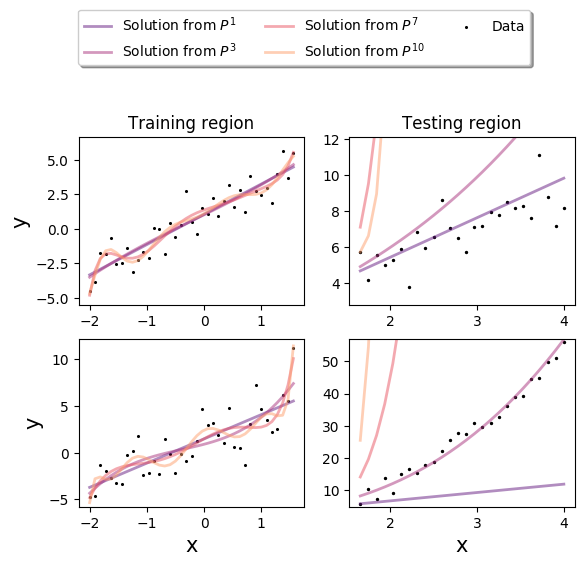
\includegraphics[width=\textwidth]{../figures/y_distr.png}
\caption{Polynomial regression of varying degrees on data drawn from a linear distribution on the left and a cubic distribution on the right. Models of varying complexity indicated by their basis $P^n$ are fit to the train data and evaluated on the test region. We observe that the higher order solutions follow what we observe to be  spurious-noise generated features in the data. This is what we call overfitting. On the right hand side we observe that the model with appropriate complexity, $f(x_i) \in P^3$, follows the true trend also in the test region while the linear and higher order models miss. The linear model does not have the capability to express the complexities of the data and is said to be underfit. Additionally we observe that the solutions of both sides degrade rapidly inside the testing region. Extending our models to previously unseen regions is very challenging.}\label{fig:overfit}
\end{figure}

\noindent To quantify the quality of the model during optimization we measure the change in the value of the cost function. In the machine learning community the best practice for this in settings were we train on tuples of response variables and data, e.g. $s_i = \{y_i, \mathbf{x}_i\}$ is to split the data in disjoint sets. From the full data one selects a subset of around $\sim 20\%$ or so that is withheld from training. After training we can evaluate the cost function on this data to create an unbiased estimate the out-of-sample error

\begin{equation}
E_{out} = C(y_{test}, f(x_{test}; \theta^*))
\end{equation}

\noindent During training we split the data yet again in two disjoint subsets, the larger of which the model is trained on. The training data gives us another measure of how good the model is, the in-sample-error, or $E_{in}$. Lastly the data that is not seen during that iteration but can be randomly selected from the train data we call validation and is our measure of when we should stop the optimization. The training error will likely decrease but for complex models this validation error $E_{val}$ will diverge and signal that the optimization should be terminated. We investigate the relationships between each of these errors and the model complexity in section \ref{sec:bv}. As to the exact size of the different partitions is largely a heuristic decision made by the amount of data available. It is also important to note that some models operate without a ground-truth labeling, or target, $y_i$. The models investigated in this thesis are either completely divorced from the ground truth variables during training or only use them in an auxiliary step. We show that this separation allows well trained models to estimate the ground truth using surprisingly few samples. 

We've conspicuously left out the fitting procedure in the paragraphs above. Generally the degree of over or under-fitting is not dependent on the fitting schema, but more on the model which we use to make predictions. In machine learning, with modern computing resources, it turns out to be much easier to make a model too complex than having it be not complex enough. \citet{Frankle2019} and \citet{Frankle2018} show that, in fact, most networks can be expressed by sub-networks contained in the modern very deep very complex neural networks. As a consequence we primarily concern ourselves then with understanding and proposing remedies to overfitting. 

The previous paragraphs contain some important features that we need to keep in mind going forward. We summarize them here for clarity: 
\begin{itemize}
\item "Fitting is not predicting" (\cite{Mehta2019}). There is a fundamental difference between fitting a model to data and making predictions from unseen samples. \\
\item Generalization is hard. Making predictions in regions of data not seen during training is very difficult, making the importance of sampling from the entire space during training that much more vital. \\
\item Complex models often lead to overfitting. While usually resulting in better results during training in the cases where data is noisy or scarce, predictions are poor outside the training sample. 
\end{itemize}
